% Your name
\renewcommand{\YRname}{R. Oechslin}

% Your grade/post
\newcommand{\YRgrade}{M2}

% Submission date
\newcommand{\YRdate}{2018.Jul.3}

% Your research theme
\newcommand{\YRtheme}{Haptic Feedback Controller with Palm Pressurization}

% Work plan
\newcommand{\YRplan}{
	\hspace{-4truemm}
	\begin{tabularx}{170truemm}{|p{50truemm}||X|X|X|X|X|X|X|X|X|X|X|X|}
		\hline
		\multicolumn{13}{|c|}{\parbox[c][10truemm][c]{0truemm}{} \large Research theme: \bf \YRtheme} \\
		\hline
		\hline
		\multicolumn{13}{|c|}{\parbox[c][8truemm][c]{0truemm}{} \large \bf --- Research Plan ---} \\
		\hline
		Term \textbackslash Month & 2 & 3 & 4 & 5 & 6 & 7 & 8 & 9 & 10 & 11 & 12 & 1 \\
		\hline
		% For ``Work plan'', do not change above.
		\hline
		Literature review & & & & & & & & & & & & \\
		\shadecells{2-2}
		\hline
		Design PlayStation Controller  & & & & & & & & & & & & \\
		\shadecells{2-3}
		\hline
		Test PlayStation Controller & & & & & & & & & & & & \\
		\shadecells{4-6}
		\hline
		Frequency Response Analysis & & & & & & & & & & & & \\
		\shadecells{5-6}
		\hline
		Design Pilot Controller & & & & & & & & & & & & \\
		\shadecells{4-6}
		\hline
		Test Pilot Controller & & & & & & & & & & & & \\
		\shadecells{6-7}
		\hline
		& & & & & & & & & & & & \\
		%\shadecells{2-10}
		\hline
		Theoretical Analysis & & & & & & & & & & & & \\
		\shadecells{6-7}
		\hline
		Analyze data and compare & & & & & & & & & & & & \\
		\shadecells{7-8}
		\hline
		Write Thesis & & & & & & & & & & & & \\
		\shadecells{8-8}
		\hline
	\end{tabularx}
}

% Main contents of your work
\newcommand{\YRachievement}{
	
	\section{Introduction}
	This report is the continuation of the first two reports about the project "Haptic Feedback Controller with Palm Pressurization". The last report has left off with the idea of implementing a voltage follower and suggested to retake measurements to create a Bode diagram. Furthermore, it has been suggested to create an analytical model and analysis of the setup in order to run simulations to identify setup parameters such as the equivalent spring constant, gain values or motor parameters.
	
	
	\section{Theoretical analysis}
	% I can check with existing papers and take their block diagram
	To come up with a theoretical analysis of the transfer function, a simplified mechanical schematic has been drawn. This schematic can be seen in figure \ref{fig:mechanical_schematic}.
	\begin{figure}[h!]
		\centering
		\includegraphics[width=0.6\linewidth]{Figs/mechanical_schematic}
		\caption{Simplified mechanical schematic of the actuation system with the stimulator.}
		\label{fig:mechanical_schematic}
	\end{figure}
	The equations of motion can be formulated with the major parameters defined in the schematic. A full explanation of all parameters can be seen in table \ref{tab:setup_params}. The variables with subscript $1$ refer to the first mass element, the carriage in its guideway, whereas variables with subscript $2$ refer to the stimulator, also known as the palm pad. For the motor the subscript $m$ has been used.
	
	\begin{figure}[h!]
		\centering
		\begin{tabular}{|l|c|c|}%designator | explanation | unit
			\hline
			 Designator & Explanation & Unit \\ \hline \hline
			$T_m$ & Motor torque & [Nm]\\ 
			$T$ & Output torque acting on carriage& [Nm]\\
			$\theta_m$ & Motor angle & [rad]\\
			$\theta$ & Clamp link angle & [rad]\\  
			$L_{CL}$ & Clamp link length & [m]\\
			$m_{1}$ & Mass of the carriage in its guideway & [kg]\\
			$m_{2}$ & Mass of the stimulator & [kg]\\
			$x_{1}$ & Position of the carriage in its guideway & [m]\\
			$x_{2}$ & Position of the stimulator & [m]\\
			$k_{eq}$ & Equivalent spring constant & [N/m]\\
			$b_{sp}$ & Spring damping coefficient & [Ns/m]\\
			$n$ & Reduction gear ratio & [-]\\
			$k_{op}$ & Spring constant of the operator & [N/m]\\
			$b_{op}$ & Damping coefficient of the operator & [Ns/m]\\
			$J_T$ & Total inertia of mechanical setup & [$\textit{kgm}^2$]\\
			\hline
		\end{tabular}
		\caption{Setup parameters}
		\label{tab:setup_params}
	\end{figure}
	
	\subsection{Assumptions}
	First of all, it is important to mention that the transfer function is non-linear, due to the motor angle $\theta_m$ that determines the force acting on the carriage with mass $m_1$. As an initial approach however, this effect has been neglected. More specifically, it is assumed that $\theta \ll 1$ and $\cos{(\theta)} \frac{T_m}{L_{CL} } = F_{carr} $ becomes $\frac{T_m}{L_{CL} } \simeq F_{carr} $. Here the angle $\theta$ is the angle of the lever, pushing the carriage (ie. $\theta_m = n \theta$). \\
	Furthermore, there are several types of friction in the system: the intrinsic friction within the motor and its reduction gear, inside the bearings and the carriage in its guideway. Additionally the springs have a non-negligible damping coefficient. In this work the overall friction and the spring damping have been merged and are represented by the friction coefficient $b_{sp}$. The stimulator, is not in contact with the controller, but with the operator. To model the damping of the skin of the operator and the friction between the skin and the palm pad, the damping coefficient $b_{op}$ has been introduced. Similarly the spring constant of the operator's skin is modeled by $k_{op}$.\\
	
	\subsection{Spring Constant and Damping Coefficient of the Operator's Hands}
	The order of magnitude of the two coefficients $k_{op}$ and $b_{op}$ are discussed in \cite{Kuchenbecker2003} \cite{Park2014} \cite{Speich2005}. They all indicate parameters varying in the same order of magnitude, namely $k_{op} \simeq 400$N/m and $b_{op} \simeq 5$Ns/m.\\
	
	\subsection{Identification of the Spring Damping Coefficient}
	The damping coefficient of the spring $b_{sp}$ can be found by comparing the theoretical results of the frequency response analysis with the experimental findings. In fact, for the experimental setup, the stimulator has been fully blocked and therefore the operator's spring coefficient can be seen as infinitely stiff.\\
	By varying $b_{sp}$ and Bode-plotting the results of the analytical transfer function, the coefficient's order of magnitude can be found. In order to do so, the analytical transfer function has to be identified.
	
	\subsection{Expected Transfer Functions}
	The system can be cut into two major transfer functions. The block diagram including these two transfer functions is depicted in figure \ref{fig:2tf_block_diagram}. 
	
	\begin{figure}[h!]
		\centering
		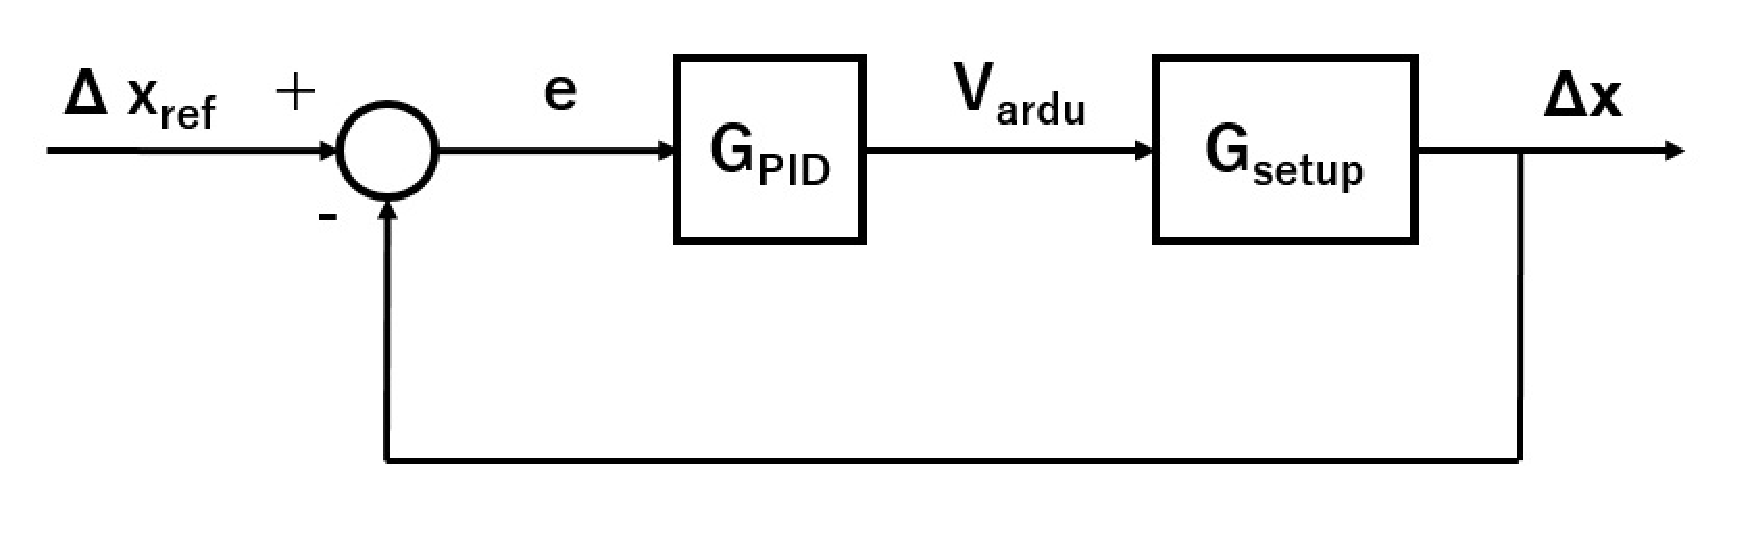
\includegraphics[width=0.6\linewidth]{Figs/2tf_block_diagram}
		\caption{Block diagram with two different transfer functions.}
		\label{fig:2tf_block_diagram}
	\end{figure}
	According to this figure one can obtain a transfer function of the following form:
	\begin{equation}
		F(s) = G_{PID}(s)G_{setup}(s) = \frac{V_{ardu}}{E}\frac{\Delta X}{V_{ardu}} = \frac{\Delta X(s)}{E(s)}
		\label{eq:complete_tf}
	\end{equation}
	where $V_{ardu}$ is the voltage output of the arduino for controlling the motors. Using this form one can calculate the individual transfer functions and finally relate the compression of the springs $\Delta x$ to the compression given as reference $\Delta x_{ref}$, since $\Delta X_{ref} / \Delta x = F/(1+F)$.
	
	\subsubsection{PID Transfer Function}
	The transfer function given by the PID-controller is very straight-forward and can be taken out of any control theory book \cite{Dutton1997}. 
	Since the arduino has limited resolution with floating point operations, the error and reference has been converted into micrometers. To keep the gains consistent between the arduino code and the matlab script for analytical analysis, the multiplication factor $K_{\mu m}$ to get from the reference distance in meters to micrometers has been introduced. Furthermore, an offset has been added ($K_{bit-offset} = 128$) to allow for negative armature voltages and lastly the PID value has been converted to the arduino output voltage, where $255$ corresponds to $5$ V. The transfer function is given in equation \ref{eq:tf_pid}. 
	\begin{equation}
		G_{PID} (s) = \frac{V_{ardu}(s)}{E(s)} = (K_{\mu m} (K_P + \frac{K_I}{s} + K_Ds) +K_{bit-offset}) K_{PID2Vardu}
		\label{eq:tf_pid}
	\end{equation}
	Finally, there is also the gain of the amplifier in voltage mode, which converts the voltage of the arduino into the voltage applied to the motors. This gain is $K_{ampl} = 10$Volt/Volt. To this voltage an offset voltage of $V_{offset} = -25$V is added.\\
	
	\subsubsection{Motor Equations}
	The second transfer function relates the motor torque $T_m$ to the arduino voltage as well as the output $\Delta x$ to $T_m$. Due to the back electromotive force these two parts are related and have to be treated as a whole.
	
	The output torque $T_m$ of the motor can be calculated using the sum of all torques and the conversion parameters intrinsic to the motor.\\
	Similar to the setup and analysis in \cite{Junior2016} the equations of the motor are given as:
	\begin{equation}
		L_a \frac{di_a}{dt} + R_a i_a + K_{emf} \dot{\theta }_m = V_a
	\end{equation}
	where $L_a$ is the armature inductance, $R_a$ the armature resistance and $i_a$ the armature current of the motor. $K_{emf}$ is the back electromotive force constant also given by the motor. $V_a$ is the armature voltage and $\theta_m$ is the angle of the motor shaft.\\
	Furthermore, with Newton's law, the sum of all torques must be zero, or:
	\begin{equation}
		J_{T} \ddot{\theta }_m - \frac{k_{eq} L_{CL}}{n} \Delta x - \frac{b_{sp} L_{CL}}{n} (\dot{x}_2 - \dot{x}_1)  = T_m = K_{\tau} i_a
		\label{eq:torques}
	\end{equation}
	In equation \ref{eq:torques} the parameter $J_{T}$ stands for the total equivalent inertia of the motor, the clamping link and the carriage of mass $m_1$.  $K_{\tau}$ is the proportional current torque gain constant. The moment of inertia can either be calculated as the sum of all inertias seen by the motor shaft, or measured in a simple test.\\ 
	
	\subsection{Analytical Inertia Identification}
	The total inertia of the system is determined by the inertia of the rotor and gears $J_m$, the inertia of the clamp link $J_{CL}$ as well as the inertia of the carriage assembly with mass $m_1$. The last one can be found by simplifying the load to a point mass at distance of the clamp link's length $L_{CL}$, which yields a moment of inertia of $J_{carr} = m_1 L_{CL}^2$.
	The gear box affects the inertia seen by the motor shaft by the square of its ratio $n$:
	\begin{equation}
		J_{reflected} = \frac{ J_{load}}{n^2}
	\end{equation}

	We therefore have a total inertia of:
	\begin{equation}
		J_T = J_m + \frac{J_{CL}}{n^2} + \frac{ m_1 L_{CL}^2}{n^2}
	\end{equation}
	where $J_{CL}$ can be calculated by approximating it as a cantilever with an off-center axis of distance $L_{CL} /2$ \footnote{(2018, June 19th) retrieved from \url{http://www.orientalmotor.com/technology/motor-sizing-calculations.html}}: %Source: http://www.orientalmotor.com/technology/motor-sizing-calculations.html
	
	\begin{equation}
		J_{CL} = \frac{1}{12}m_{CL}(A^2 + B^2 + 12l^2)
	\end{equation}
	where $A$ and $B$ are the width and length respectively.\\
	The calculated total moment of inertia for the motor with a reduction ration of $n = 112$ is $J_T = 6.87 \times 10^{-8}$ $\textit{kgm}^2$.
	
	\subsection{Experimental Inertia Identification}
	Alternatively, one can approximate the total moment of inertia by applying a constant current on the motor and measuring the acceleration. In this case the traveled distance has been derivated twice to find the acceleration, which results in an amplification of errors. Furthermore, the constant current has been kept very low, (between $20$ and $100$ mA), which led to a slow movement and therefore higher friction impact on the measurements. However, the results are consistent with the theoretically calculated values:
	$$ J_T = \frac{7.5 \times 10^{-4}}{n^2} = 5.98 \times 10^{-8} \textit{ kgm}^2$$ 
	
	\subsection{Relating $\Delta X$ to $\theta$}
	The conversion between the angle $\theta$ and the carriage's traveled distance $x_1$ can be found by assuming that the horizontal displacement of the carriage is given by $L_{CL} sin(\theta) = x_1$. For small angles of $\theta$ the Taylor expansion gives:
	\begin{equation}
		L_{CL} \theta \simeq x_1
		\label{eq:assum}
	\end{equation} 
	
	The output $\Delta x$ is the compression of the springs and is given by $\Delta x = x_2 - x_1$. For finding $x_2$ the equation of motion given by Newton's law has been considered.
	
	\begin{equation}
		m_2 \ddot{x}_2 = -k_{eq} (x_2 - x_1) - b_{sp} (\dot{x}_2 - \dot{x}_1) - k_{op} x_2 - b_{op} \dot{x}_2
		\label{eq:mov_stimul}
	\end{equation}
	In the case where the stimulator has been blocked by a wall, $\dot{x}_2$ has been forced to zero. Using the Laplace transform and equation \ref{eq:mov_stimul} one finds the expression of $x_2$:
	
	\begin{equation}
		X_2 = -\frac{k_{eq} + b_{sp} s}{s^2 m_2 + b_{op} s + k_{op}} \Delta X
		\label{eq:x2dx}
	\end{equation}
	
	\subsubsection{Motor and Spring Transfer Function}
	Combining all the equations one can find the final block diagram, which can be seen in figure \ref{fig:block_diagram}
	\begin{figure}[h!]
		\centering
		\includegraphics[width=0.95\linewidth]{Figs/block_diagram}
		\caption{Complete block diagram relating the output $\Delta x$ to the input $\Delta x_{ref}$.}
		\label{fig:block_diagram}
	\end{figure}


	From this diagram and the equations mentioned above, one can obtain the transfer functions that relate the output $\Delta x$ and input $\Delta x_{ref}$ as introduced in equation \ref{eq:complete_tf},
	where $\Delta X(s)$ and $\Delta X_{ref}(s)$ are the Laplace transforms of the output and input functions respectively. \\
	It is thus possible to study the frequency response by simulating this setup with the assumptions mentioned earlier.
	
	\subsection{Main Equations for Analytical Transfer Function}
	\begin{equation}
		\Delta X_{ref} - \Delta X = E
		\label{eq:error}
	\end{equation}
	
	\begin{equation}
		((K_P + K_D s + \frac{K_I}{s})E K_{\mu m} + K_{bit-offset}) K_{PID2Vardu} K_{ampl} + V_{offset}= V_a
		\label{eq:PID}
	\end{equation}
	
	\begin{equation}
		\frac{V_a - K_{emf}\dot{\theta}_m}{L_a s + R_a} K_{\tau} + F_{coupled} = J_T \ddot{\theta}_m
		\label{eq:motor_torques}
	\end{equation}
	
	\begin{equation}
		F_{coupled} = (k_{eq} + b_{sp}s) \frac{L_{CL}}{n} \Delta X
		\label{eq:fcoupled}
	\end{equation}
	
	\begin{equation}
		\theta_m = \frac{n}{L_{CL}} X_1 = -\frac{n}{L_{CL}}(1 + \frac{k_{eq} + b_{sp}s}{m_2 s^2 + b_{op}s + k_{op}}) \Delta X
	\label{eq:theta}
	\end{equation}
	
	Note that the constant offsets in equation \ref{eq:PID} are for pure symmetrical reasons and will cancel each other out, since $K_{bit-offset} K_{PID2Vardu} K_{ampl} + V_{offset} = 0$ and the equation becomes $ ((K_P + K_D s + \frac{K_I}{s})E K_{\mu m} ) K_{PID2Vardu} K_{ampl}= V_a$. This is the equivalent to a standard PID form with gains $K'_P$, $K'_D$ and $K'_I$.\\
	In the case of the experimental setup the palm pad has been blocked and therefore $x_2$ has been forced to be constant. The last equation becomes thus: $\theta_m = - \frac{n}{L_{CL}} \Delta X$.
	
	\subsection{Tracking Behavior of the P-controller}
	The tracking behavior of the P-controlled setup can be seen in the following figures.
	\begin{figure}[h!]
		\centering
		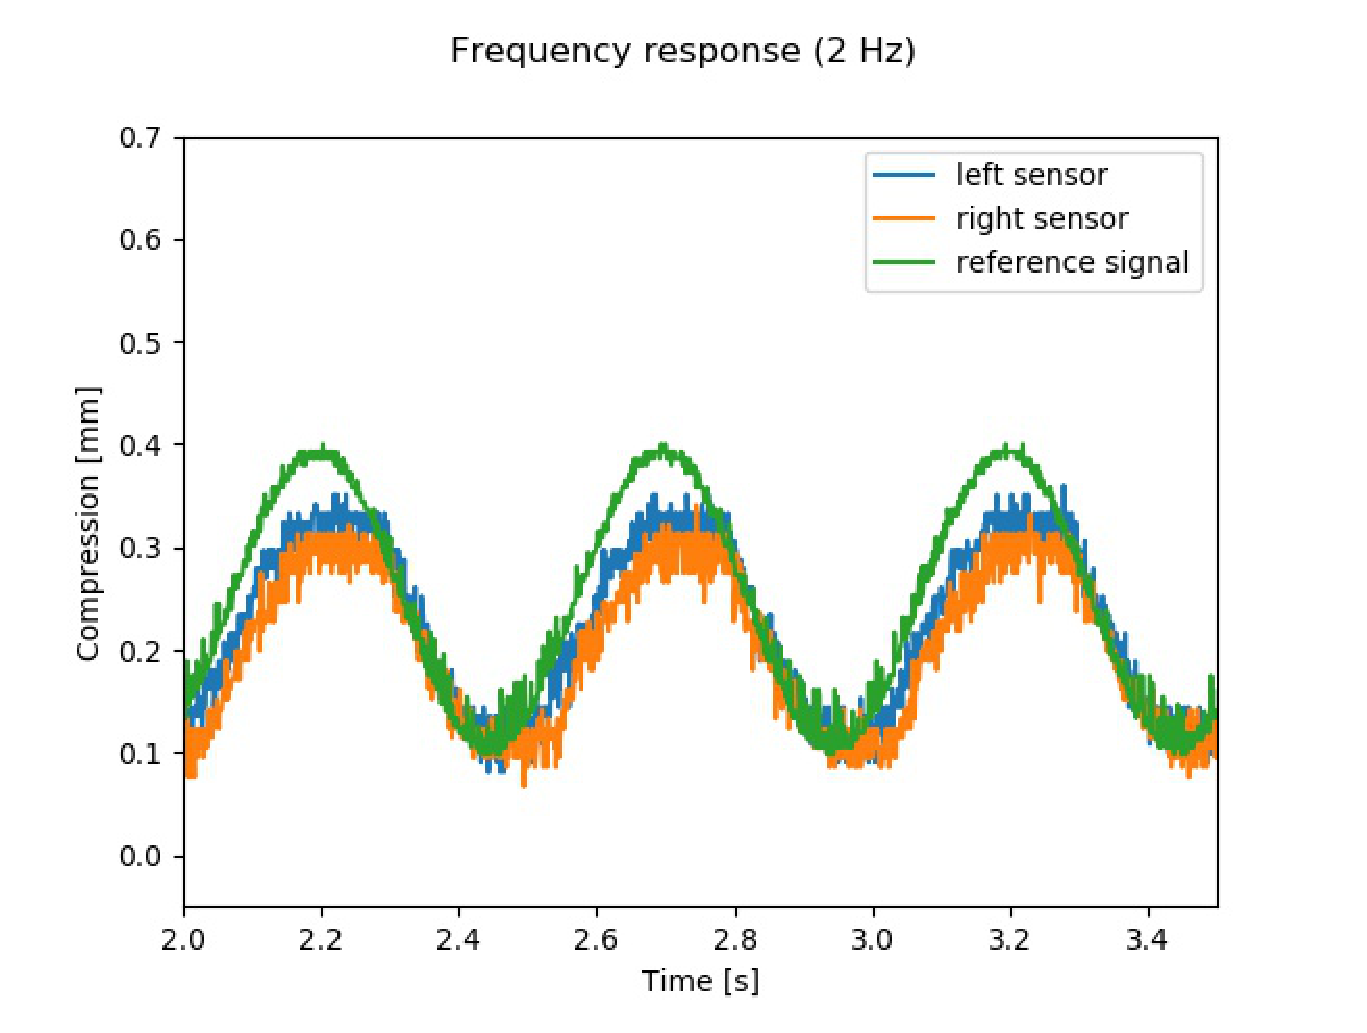
\includegraphics[width=0.6\linewidth]{Figs/2plot_zoom_P}
		\caption{Tracking behavior of the P-controller for $2$ Hz.}
		\label{fig:2plot_zoom_P}
	\end{figure}
	\begin{figure}[h!]
		\centering
		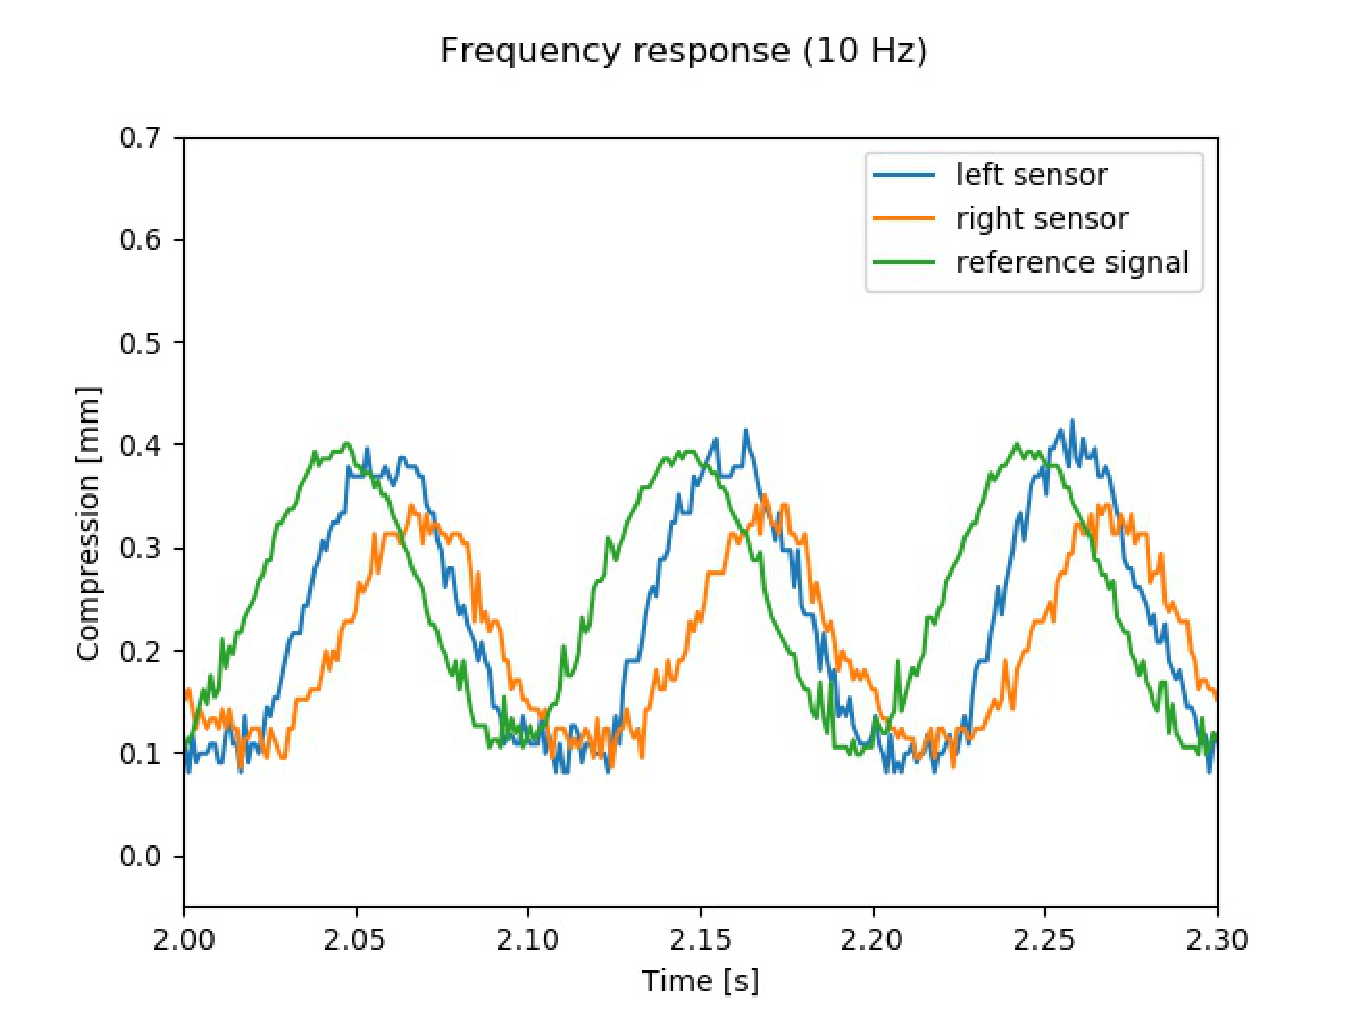
\includegraphics[width=0.6\linewidth]{Figs/10plot_zoom_P}
		\caption{Tracking behavior of the P-controller for $10$ Hz.}
		\label{fig:10plot_zoom_P}
	\end{figure}
	
	%show picture, explain problem of steady state offset, find PID values
	
	\subsection{Comparison of Results - P-controller and Experimental Data}
	The analytical transfer function has only been calculated for a specific set of spring damping coefficients $b_{sp}$. The results for the uniformly spaced values between $100$Ns/m and $400$Ns/m are depicted in figure \ref{fig:bode_all_combined_P02}. The gains that have been used are for a P-controller, it was namely $K_P' = 39.2 \frac{\textit{V}}{\textit{mm}}$. The simulation result that was closest to the experimental setup can be seen in figure \ref{fig:bode_sp_damp300_P02} and the corresponding transfer function is:
	\begin{equation}
		%\frac{\Delta X}{\Delta X_{ref}} = \frac{7.04\times 10^{-3} s^2 + 288 s + 2.94\times 10^{6}}{1.09\times 10^{-10}s^5 + 6.69\times 10^{-6}s^4 + 0.137 s^3 + 940s^2 +6.45 s + 2.95\times 10^{6}}
		\frac{\Delta X}{\Delta X_{ref}} = \frac{1.23 \times 10^3}{3.24\times 10^{-6}s^3 + 6.67\times 10^{-2}s^2 + 8.48s + 1.23 \times 10^3}
	\end{equation}
	

\begin{figure}[h!]
	\centering
	\includegraphics[width=0.6\linewidth]{Figs/bode_all_combined_P02}
	\caption{Bode plot comparison of experimental data of the P-controller and analytical transfer functions for several different $b_{sp}$.}
	\label{fig:bode_all_combined_P02}
\end{figure}

\begin{figure}[h!]
	\centering
	\includegraphics[width=0.6\linewidth]{Figs/bode_sp_damp300_P02}
	\caption{Bode plot comparison of experimental data of the P-controller and analytical transfer function for $b_{sp} = 300$Ns/m.}
	\label{fig:bode_sp_damp300_P02}
\end{figure}

%	\begin{figure}[h!]
%		\centering
%		\begin{subfigure}{.5\textwidth}
%			\centering
%			\includegraphics[width=0.6\linewidth]{Figs/bode_all_combined_P02}
%			\caption{Bode plot comparison of experimental data of P-controller and analytical transfer functions for several different $b_{sp}$.}
%			\label{fig:bode_all_combined_P02}
%		\end{subfigure}%
%		\begin{subfigure}{.5\textwidth}
%			\includegraphics[width=0.6\linewidth]{Figs/bode_sp_damp300_P02}
%			\caption{Bode plot comparison of experimental data of P-controller and analytical transfer function for $b_{sp} = 300$Ns/m.}
%			\label{fig:bode_sp_damp300_P02}
%		\end{subfigure}
%		%\caption{A figure with two subfigures}
%		%\label{fig:test}
%	\end{figure}



As it can be seen in figure \ref{fig:bode_sp_damp300_P02} there is a constant gain of $1$ for lower frequencies and a slight resonance top becomes visible around $18$Hz. The phase shift is of around $-210^\circ$ for the tested frequencies, and the lag does not increase more than $45 ^\circ$ for the frequencies of interest. Due to the setup constraints, the analytical results of higher frequencies have not been considered.

\subsection{Motor Comparison}
When one goes back to the experimental results where the two motors with different reduction gear ratios have been compared (previous report), %TODO make reference here, put up to date photos
one can conclude that the motor with the higher reduction ratio has a higher output force with a tradeoff of speed. Since one of the critical elements of the SEA system is its actuation speed, it is essential to push the boundaries as far as possible. However, the high gain frequency response in the experimental setup starts to drop at much higher frequencies than the actual operating frequency (which is given by the rather slow communication speed between the robot and the control device of $f_{op} \simeq 2-5$ Hz).\\
Due to the fact that even with the stronger reduction gear motor, the springs cannot be compressed to their limits, a higher possible output force has been favored and therefore the stronger motor seems more appropriate.

\subsection{Experimental PID Tuning}
At first, the Ziegler Nichols tuning method has been used to identify the PID gains for the setup. However, due to the non-linear behaviour, these gains resulted in a rather poor tracking performance of the reference signal.\\
Since an educated tuning of the gains is the very core problem of all control engineering, a lot of different approaches exist to find optimal or sub-optimal gain values. Given the complexity of the setup, it seemed reasonable to go for the simple trial and error approach, where the gains have been tuned and the tracking performance was shown in real-time. This approach led to the following gain coefficients:

%TODO discuss the fact of neglected efficiency, what is backdriveability exactly, redo bode plot with new pid settings 
\begin{figure}[h!]
	\centering
	\begin{tabular}{|l|c|c|}
		\hline
		Designator & Value & Unit \\ \hline \hline
		$K'_P$ & $47.6$ & [V/mm]\\ 
		$K'_I$ & $0.124$ & [V/mm/s]\\
		$K'_D$ & $247$ & [Vs/mm]\\
		\hline
	\end{tabular}
	\caption{Trial and error PID tuning.}
	\label{tab:trial_error_pid}
\end{figure}


\subsection{Tracking Behavior of the PID-controller}
The tracking behavior of the P-controlled setup can be seen in the following figures.
%show picture, explain problem of steady state offset, find PID values
\begin{figure}[h!]
	\centering
	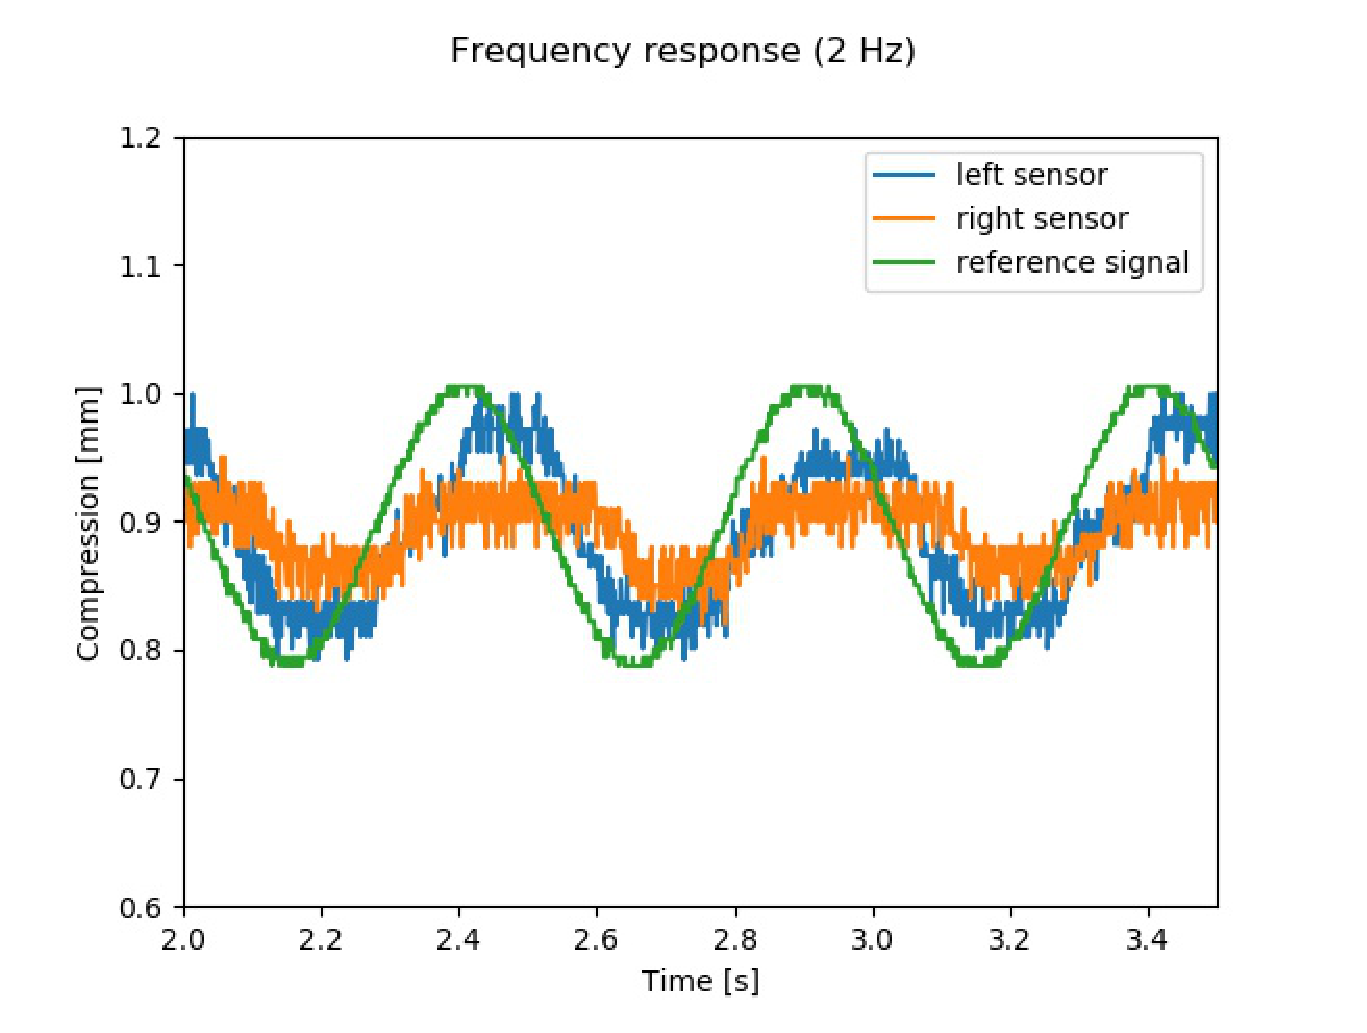
\includegraphics[width=0.6\linewidth]{Figs/2plot_zoom_PID}
	\caption{Tracking behavior of the PID-controller for $2$ Hz.}
	\label{fig:2plot_zoom_PID}
\end{figure}
\begin{figure}[h!]
	\centering
	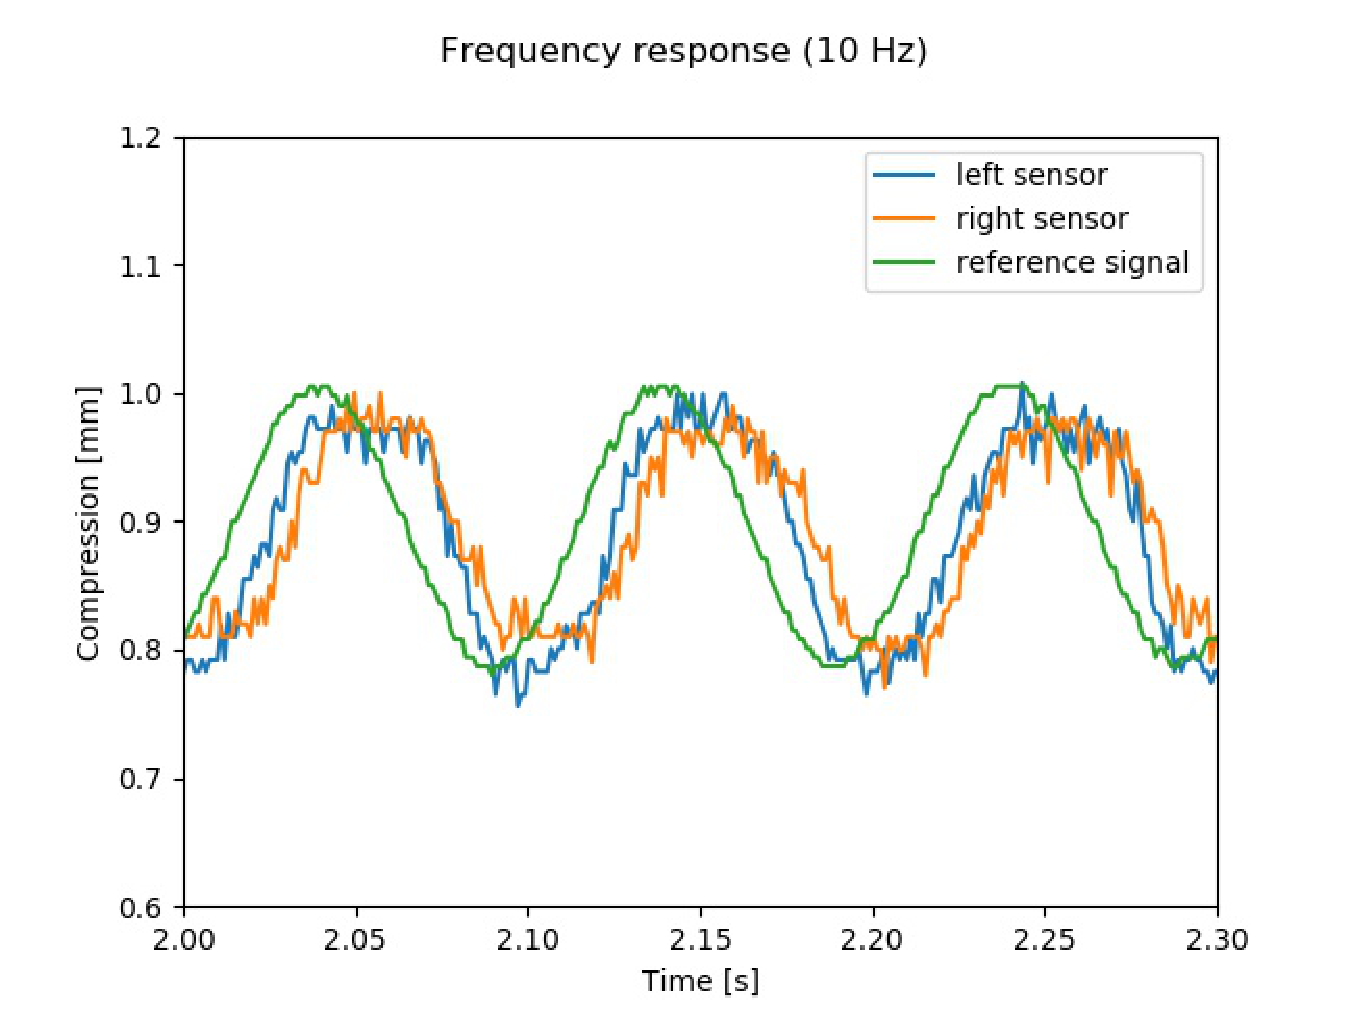
\includegraphics[width=0.6\linewidth]{Figs/10plot_zoom_PID}
	\caption{Tracking behavior of the PID-controller for $10$ Hz.}
	\label{fig:10plot_zoom_PID}
\end{figure}

\subsection{Comparison of Results - PID-controller and Experimental Data}
With the gains stated in table \ref{tab:trial_error_pid}, the frequency response can be measured again. This has been done for the left and right side, both using the motor with a reduction ratio of $n = 112$. The comparison between the analytical results from the mathematical model and the experimentally gathered data can be seen in figure \ref{fig:bode_sp_damp100_PID}.

\begin{figure}[h!]
	\centering
	\includegraphics[width=0.6\linewidth]{Figs/bode_sp_damp100_PID}
	\caption{Bode plot comparison of experimental data of the PID-controller and analytical transfer function for $b_{sp} = 100$Ns/m.}
	\label{fig:bode_sp_damp100_PID}
\end{figure}



\section{Discussion}
\subsection{P-controlled Device}
As figure \ref{fig:bode_sp_damp300_P02} indicates, the results of the mathematical model seems to correspond with the experimental data. Furthermore, a damping coefficient of $b_{sp} = 300$ Ns/m could be identified. The tracking behavior of this P-controller was reasonable for lower frequencies, even though there was a slight steady-state offset. The constant phase-lag was very small for small frequencies and did not exceed $45^\circ$ for frequencies up to $10$ Hz. Even an approach of discretizing the analytical results did not yield a better match of the results. %TODO necessary to discuss this, or show the graph?
 
\subsection{PID-controlled Device}
When the PID-controller has been implemented, the difference between analytical results and the experiments was much bigger. First it was noteworthy, that the two motors showed a different behavior with the same gains. This might stem from several asymmetries in the setup. First of all and most importantly, the distance sensors are different, and have different threshold values. Also, the springs might not have been glued in a perfectly symmetrical manner. However, the noise characteristics of the sensors are in a similar order of magnitude and do not account for the differences here. Lastly, there are the mechanical aspects of how the motors have been screwed to the controller. Due to the high-frequency driving, the screws loosen from time to time, which can have a significant impact on the Bode plots. Furthermore, there might be a slight misalignment of the motor shaft axis and the guideway, which results in an opposing force.\\
Again, the discretization of the analytical transfer function did not yield a better match between the analytical and experimental data.\\
Judging from the frequency response seen in figure \ref{fig:bode_sp_damp100_PID} the tracking is relatively bad at low frequencies, not only because there is an attenuation, but also that the resonance top at higher frequencies quickly leads to saturation of the applicable motor voltage. In addition to this, the phase lag is much bigger and is already at least $45 ^\circ$ in the lower range of the bandwidth. This is due to the filters that have been used. The first filter is an RC-circuit that takes the PWM signal from the arduino and produces a more continuous voltage signal for the amplifiers. The cut-off frequency is $330$ Hz. The second filter is within the arduino code and is used to filter the measured distance. This filter was necessary to reduces the impact of noise amplification in the derivative part of the PID-controller. Three different filters with cut-off frequencies from $f_1 = 1.6$ Hz, $f_2 = 4.2$ Hz and $f_3 = 8.8$ Hz have been tested.

% talk about filter and filter impact, problem of discretization, results	

\section{Conclusion}
Given the results for the P-controller, one can assume that the mathematical model is correct. However, when one implements a PID-controller, a higher discrepancy between mathematical model and experimental data arises. Even though the parameters used in the mathematical model have been double-checked (such as the moment of inertia for example), its validity can be questioned.\\
From the two different implementations, the P-controller shows a better tracking behavior for the operational bandwidth.

\section{Outlook}
In the future, the P- and PID-controller shall be tested and a subjective measure of the feedbacks smoothness and transparency shall be reported.\\
A more thorough literature shall be done to discuss the findings with existing papers.\\
A design-choice guide shall be created in order to facilitate future research for similar setups.


	
	%�����܂�
}


